\section{Creando Proyecto con Maven}
\label{proyMaven}

En esta sección se mostrará el paso a paso para crear desde Visual Studio Code un proyecto Maven para ANTLR4.  Al finalizar el procedimiento, tendremos el primer proyecto listo para usar.

\subsection{Creación del Proyecto}
\label{creacionProy}

Para crear el proyecto, se debe acceder al \emph{Command Palette} con las teclas \verb|Ctl+Shift+p| y comenzar a teclear la palabra ``Maven''. Elegir la opción \emph{``Maven: Create Maven Project''} (Fig.~\ref{mavenNuevo}).

Maven ofrece varios arquetipos para tomar como estructura del proyecto.  Vamos a elegir el \emph{``maven-archetype-quickstart''} (Fig.~\ref{mavenArch}), verión 1.4, porque genererá un proyeto simple que luego configuraremos a nuestra necesidad.  La configuración del proyecto se encuentra en el archivo \verb|pom.xml|.

Hecho esto, nos pedirá que indiquemos el directorio donde se creará el proyecto.  En el directorio indicado, se creará un nuevo directorio con el nombre del proyecto.

\begin{figure}[t]
	\centering
	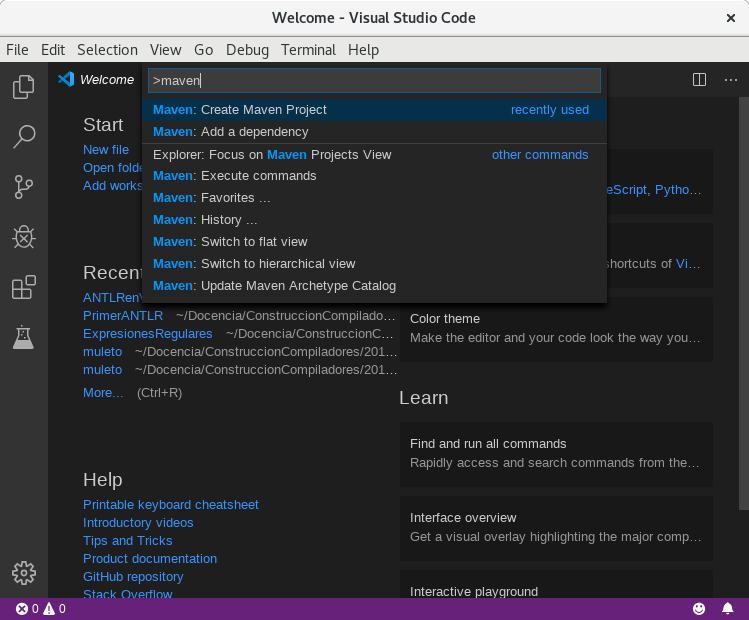
\includegraphics[width=.95\textwidth]{img/CrearMavenProject}
	\caption{Nuevo proyecto Maven.}
	\label{mavenNuevo}
\end{figure}

\begin{figure}[t]
	\centering
	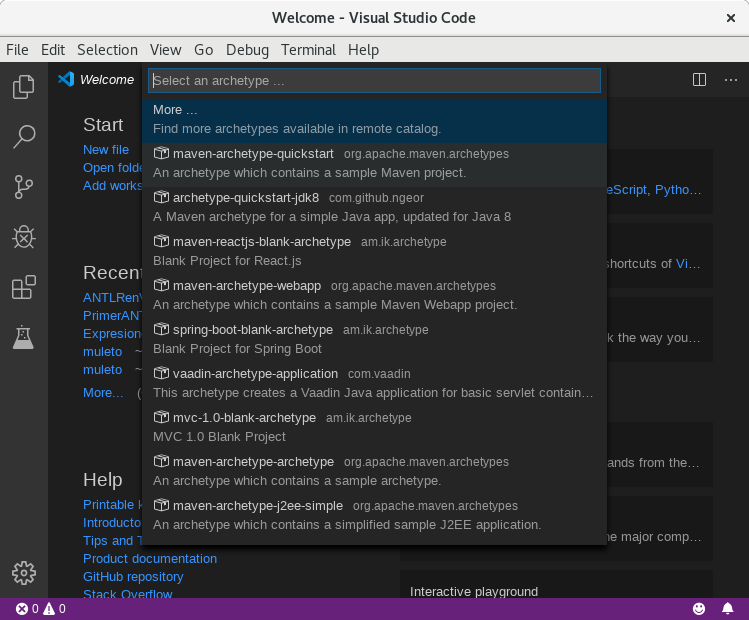
\includegraphics[width=.95\textwidth]{img/MavenArchetypeSample}
	\caption{Arquetipo Maven para Java.}
	\label{mavenArch}
\end{figure}

Finalmente, nos pedirá de forma interactiva en la terminal, que ingresemos datos del proyecto. Se pueden aceptar la mayor parte de la sugerencias, pero lo importante es indicar correctamente el \verb|groupID| y el \verb|artifactID|.  En nuestro caso, usaremos \verb|PrimerProyecto| para ambos campos.  El directorio del proyecto se corresponde con el \verb|groupID|.  Para más información sobre nombres de proyectos ver la documentación en la página de \href{https://maven.apache.org/guides/mini/guide-naming-conventions.html}{Maven}.

\begin{figure}[t]
	\centering
	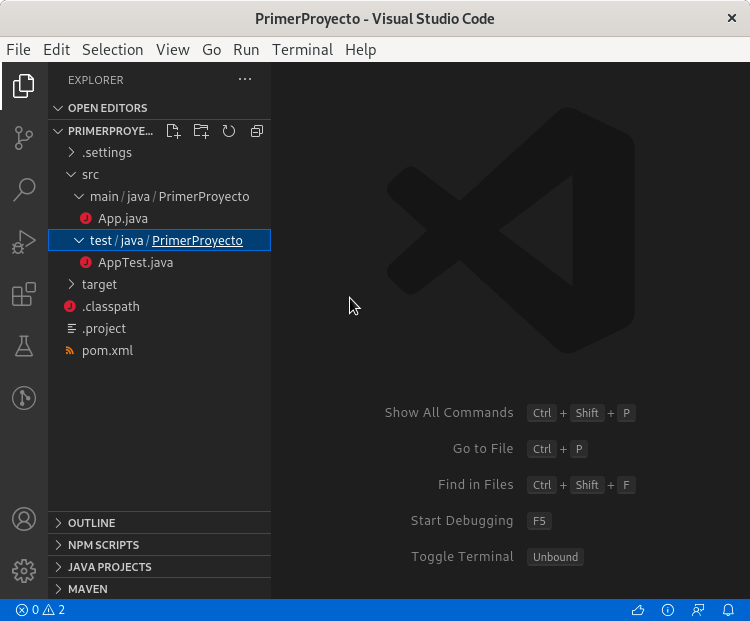
\includegraphics[width=.95\textwidth]{img/MavenProjectoCreado}
	\caption{Proyecto Maven para Java recién creado.}
	\label{mavenSinConf}
\end{figure}

Si el proceso termina correctamente obtendremos un \emph{``Build success''}.  El proyecto no se abre automáticamente, por lo tanto, hay abrirlo desde el menú ``File'' con la opción ``Open Folder'' o usar la combinación de teclas \verb|Ctl+K Ctl+O|.  El proyecto se verá como en la Fig.~\ref{mavenSinConf}.


\subsection{Configuración para Java~11}
\label{mavenJava}

\lstinputlisting[float,style=miXML,caption={Sección \texttt{properties} del archivo \texttt{pom.xml}.},label=pomJava]{code/Java11pom.xml}

Para indicar la versión correcta de Java a usar, debemos editar el archivo \verb|pom.xml|. En la sección \verb|properties| pondremos el número de versión Java como puede verse en el Código~\ref{pomJava}.
    
\begin{figure}[t]
	\centering
	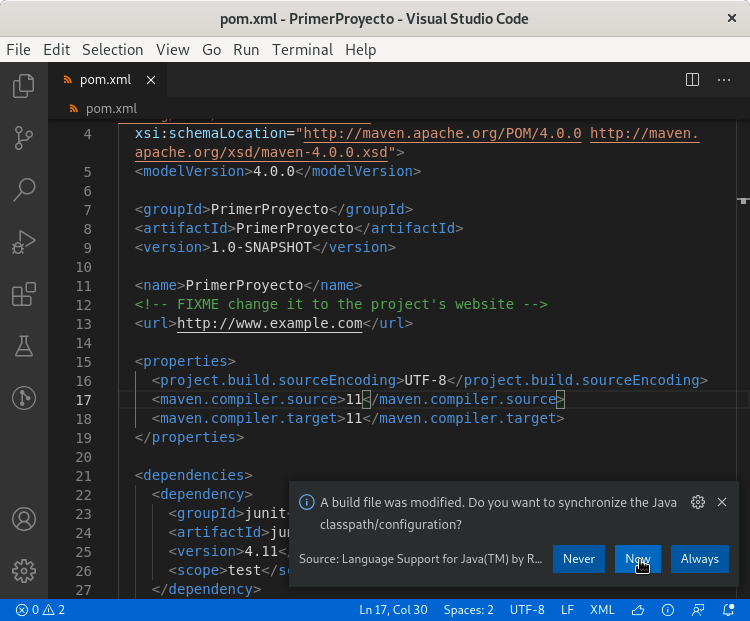
\includegraphics[width=.95\textwidth]{img/MavenPomActualizar}
	\caption{Actualizar configuración proyecto Maven.}
	\label{mavenActConf}
\end{figure}

Al grabar el archivo, se detectará el cambio y preguntará si se desea actualizar la configuración del proyecto (Fig.~\ref{mavenActConf}).  Al aceptar, se podrá ejecutar el proyecto abriendo el archivo \verb|App.java| para verificar la correcta configuración (Fig.~\ref{mavenTestEx}).  Si no encontramos ningún inconveniente, entonces el proyecto se encuentra listo para usar Java~11.


\subsection{Configuración para ANTLR4}
\label{mavenANTLR}

\lstinputlisting[float,style=miXML,caption={Sección \texttt{dependency} del archivo \texttt{pom.xml}.},label=pomANTLR]{code/ANTLRpom.xml}

\begin{figure}[t]
	\centering
	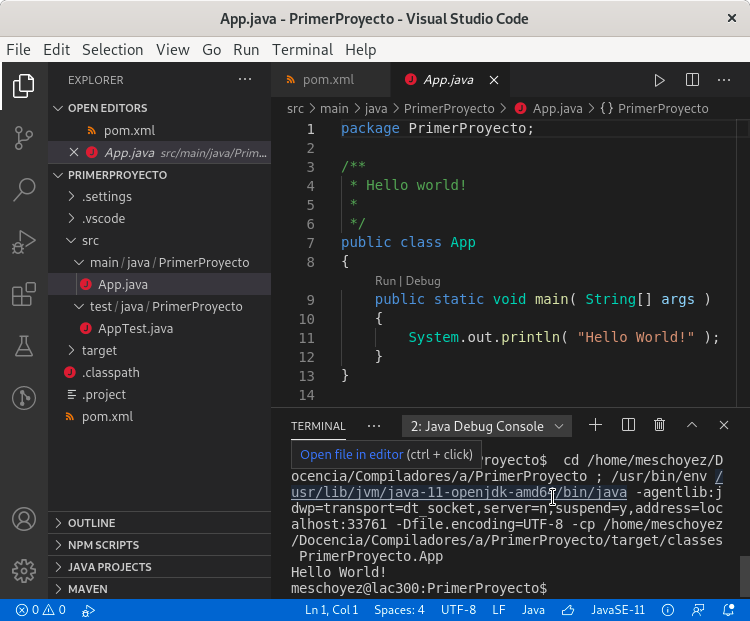
\includegraphics[width=.95\textwidth]{img/MavenTestEx}
	\caption{Prueba configuración del proyecto Maven para Java.}
	\label{mavenTestEx}
\end{figure}

Los gestores de proyectos tienen, entre otros objetivos, resolver las dependencias necesarias para la compilación y ejecución del software con las diferentes bibliotecas de software.  Para usar ANTLR4, debemos configurar su dependencia en el archivo \verb|pom.xml|.  El Código~\ref{pomANTLR} se copió de \href{https://mvnrepository.com/artifact/org.antlr/antlr4}{MVNRepository}.

Finalizados los pasos indicados, tenemos listo el proyecto Maven para compilar en Java un software que utiliza ANTLR4.  En la próxima sección abordaremos como configurar el \emph{plug--in} de ANTLR.
